\documentclass[11pt]{article}

%% -- LaTeX packages --
\usepackage[utf8]{inputenc}
\usepackage[T1]{fontenc}
\usepackage{lmodern}
\usepackage{amsmath,amssymb}
\usepackage{graphicx}
\usepackage{booktabs}
\usepackage{hyperref}
\usepackage{natbib}
\usepackage[margin=1in]{geometry}
\usepackage{xcolor}

%% Custom commands for JSS-style markup
\newcommand{\proglang}[1]{\textsf{#1}}
\newcommand{\pkg}[1]{\textbf{#1}}
\newcommand{\code}[1]{\texttt{#1}}
\newcommand{\fct}[1]{\code{#1()}}
\newcommand{\class}[1]{`\code{#1}'}

%% Title and authors
\title{\pkg{RcppML}: High-Performance Non-Negative Matrix Factorization\\
with Cross-Validation for \proglang{R}}

\author{Zachary DeBruine\\
Department of Computational Medicine and Bioinformatics\\
University of Michigan\\
\texttt{debruine@umich.edu}}

\date{}

\begin{document}

\maketitle

\begin{abstract}
Non-negative matrix factorization (NMF) is a fundamental dimensionality 
reduction technique with applications spanning bioinformatics, text mining, 
computer vision, and signal processing. This paper presents \pkg{RcppML}, an 
\proglang{R} package that implements a comprehensive NMF framework with several 
key innovations: (1) a highly optimized sequential coordinate descent solver for 
non-negative least squares with support for L1 regularization and bounded 
solutions; (2) streaming cross-validation with minimal computational overhead 
using a novel position-dependent random number generator; (3) multiple robust 
loss functions including MSE, MAE, Huber, and KL-divergence implemented via 
iteratively reweighted least squares; (4) automatic rank determination through 
golden section search optimization; (5) specialized rank-2 NMF for 
high-performance spectral bipartitioning. The package provides unified support 
for both sparse and dense matrices through template metaprogramming and achieves 
state-of-the-art performance through careful cache-aware algorithm design.

\vspace{1em}
\noindent\textbf{Keywords:} non-negative matrix factorization, cross-validation, coordinate 
descent, spectral clustering, \proglang{R}, \proglang{C++}, \pkg{Rcpp}
\end{abstract}


%% =============================================================================
\section{Introduction} \label{sec:introduction}

Non-negative matrix factorization (NMF) decomposes a non-negative matrix 
$\mathbf{A} \in \mathbb{R}_{\geq 0}^{m \times n}$ into two non-negative factor 
matrices $\mathbf{W} \in \mathbb{R}_{\geq 0}^{m \times k}$ and 
$\mathbf{H} \in \mathbb{R}_{\geq 0}^{k \times n}$ such that 
$\mathbf{A} \approx \mathbf{W}\mathbf{H}$ \citep{Lee1999}. The non-negativity 
constraints enable parts-based, interpretable representations that have proven 
valuable across diverse domains including facial recognition \citep{Lee1999}, 
text mining \citep{Xu2003}, gene expression analysis \citep{Brunet2004}, and 
single-cell genomics \citep{Kotliar2019}.

Despite its widespread use, practical NMF deployment faces several challenges. 
First, selecting the factorization rank $k$ is critical but often performed 
heuristically or through computationally expensive techniques like consensus 
clustering \citep{Brunet2004}. Second, NMF optimization is sensitive to outliers 
when using standard squared error loss. Third, achieving high performance 
requires careful algorithm engineering, particularly for sparse data common in 
modern applications.

The \pkg{RcppML} package for \proglang{R} addresses these challenges through 
several key contributions:

\begin{enumerate}
  \item \textbf{Integrated cross-validation}: A streaming algorithm that 
  computes held-out reconstruction error with minimal overhead ($<$5\% typical), 
  enabling principled rank selection without external validation frameworks.
  
  \item \textbf{Robust loss functions}: Support for MSE, MAE, Huber, and 
  KL-divergence losses implemented via iteratively reweighted least squares 
  (IRLS), providing robustness to outliers and flexibility for different data 
  types.
  
  \item \textbf{Automatic rank determination}: Golden section search 
  optimization over the cross-validation objective to automatically identify 
  optimal rank.
  
  \item \textbf{Specialized rank-2 NMF}: A highly optimized implementation for 
  spectral bipartitioning that outperforms truncated SVD approaches.
  
  \item \textbf{High-performance implementation}: Cache-aware sequential 
  coordinate descent with unified support for sparse and dense matrices through 
  \proglang{C++} template metaprogramming.
\end{enumerate}

The package is implemented as a header-only \proglang{C++} library integrated 
with \proglang{R} through \pkg{Rcpp} \citep{Eddelbuettel2011, Eddelbuettel2013}. 


%% =============================================================================
\section{NMF algorithm} \label{sec:algorithm}

\subsection{Problem formulation}

We formulate NMF with a scaling diagonal that separates factor magnitude from 
factor direction. Given $\mathbf{A} \in \mathbb{R}_{\geq 0}^{m \times n}$, we 
seek:
\begin{equation}
  \min_{\mathbf{W}, \mathbf{D}, \mathbf{H}} 
  \mathcal{L}(\mathbf{A}, \mathbf{W}\mathbf{D}\mathbf{H}) + 
  \lambda_1 \|\mathbf{W}\|_1 + \lambda_1 \|\mathbf{H}\|_1
  \label{eq:objective}
\end{equation}
subject to $\mathbf{W}, \mathbf{H} \geq 0$, $\mathbf{D} = \text{diag}(d_1, 
\ldots, d_k)$, and optional column normalization $\|\mathbf{w}_j\|_2 = 1$.

The diagonal scaling $\mathbf{D}$ provides several benefits: (1) it decouples 
factor magnitude from direction, improving convergence; (2) it enables 
consistent comparison across runs with different initializations; (3) it 
facilitates L1 regularization by normalizing factor scales.

\subsection{Alternating least squares}

We optimize Equation~\ref{eq:objective} using alternating least squares (ALS), 
iteratively solving:
\begin{align}
  \mathbf{H} &\leftarrow \arg\min_{\mathbf{H} \geq 0} 
  \|\mathbf{A} - \mathbf{W}\mathbf{D}\mathbf{H}\|_F^2 + \lambda_1\|\mathbf{H}\|_1 
  \label{eq:h_update} \\
  \mathbf{W} &\leftarrow \arg\min_{\mathbf{W} \geq 0} 
  \|\mathbf{A}^\top - \mathbf{H}^\top\mathbf{D}\mathbf{W}^\top\|_F^2 + 
  \lambda_1\|\mathbf{W}\|_1
  \label{eq:w_update}
\end{align}

Each subproblem decomposes into independent non-negative least squares (NNLS) 
problems over columns. For the $\mathbf{H}$ update, letting 
$\tilde{\mathbf{W}} = \mathbf{W}\mathbf{D}$, we solve for each column $j$:
\begin{equation}
  \mathbf{h}_j \leftarrow \arg\min_{\mathbf{h} \geq 0} 
  \|\mathbf{a}_j - \tilde{\mathbf{W}}\mathbf{h}\|_2^2 + \lambda_1\|\mathbf{h}\|_1
  \label{eq:nnls}
\end{equation}

\subsection{Sequential coordinate descent solver}

We solve Equation~\ref{eq:nnls} using sequential coordinate descent 
\citep{Franc2005}. The algorithm iteratively updates each coordinate while 
holding others fixed:
\begin{equation}
  h_i \leftarrow \max\left(0, \frac{\mathbf{w}_i^\top(\mathbf{a} - 
  \tilde{\mathbf{W}}\mathbf{h}) + h_i \|\mathbf{w}_i\|_2^2 - \lambda_1}
  {\|\mathbf{w}_i\|_2^2}\right)
  \label{eq:cd_update}
\end{equation}

The key insight is to maintain the residual $\mathbf{r} = \mathbf{a} - 
\tilde{\mathbf{W}}\mathbf{h}$ incrementally. After updating $h_i$ to 
$h_i^{\text{new}}$, we update:
\begin{equation}
  \mathbf{r} \leftarrow \mathbf{r} - (h_i^{\text{new}} - h_i)\mathbf{w}_i
\end{equation}

This reduces the complexity of each coordinate update from $O(mk)$ to $O(m)$, 
making the overall NNLS solve $O(mk)$ per column.


%% =============================================================================
\section{Cross-validation framework} \label{sec:crossvalidation}

\subsection{Motivation}

Selecting the factorization rank $k$ is a fundamental challenge in NMF. 
Cross-validation provides a principled alternative to heuristics: hold out a 
random subset of entries, fit NMF on the observed entries, and evaluate 
reconstruction error on the held-out entries.

\subsection{Zero-masking for sparse matrices}

For sparse data, we only mask non-zeros---zeros are uninformative since NMF 
naturally predicts small values for unobserved entries. Let $\Omega$ denote 
the set of observed (non-zero) entries and $\Omega_{\text{test}} \subset \Omega$ 
denote the held-out test set. The test error is:
\begin{equation}
  \text{MSE}_{\text{test}} = \frac{1}{|\Omega_{\text{test}}|} 
  \sum_{(i,j) \in \Omega_{\text{test}}} (A_{ij} - [\mathbf{W}\mathbf{D}
  \mathbf{H}]_{ij})^2
\end{equation}

\subsection{Position-dependent random masking}

We use a position-dependent random number generator that deterministically 
determines whether each entry is masked based on its position $(i, j)$:
\begin{equation}
  \text{mask}(i, j) = \mathbf{1}[\text{hash}(i, j, \text{seed}) < p_{\text{cv}}]
\end{equation}

This ``speckled'' RNG has several advantages: (1) no memory allocation for the 
mask; (2) the same entry maps to the same mask value throughout optimization; 
(3) reproducibility through the seed.

\subsection{Streaming loss accumulation}

During each ALS iteration, we accumulate test error ``for free'' within the 
NNLS solve by checking the mask and accumulating squared residuals during 
the normal computation. This streaming approach has $O(1)$ memory overhead.


%% =============================================================================
\section{Loss functions} \label{sec:lossfunctions}

\pkg{RcppML} supports four loss functions via iteratively reweighted least 
squares (IRLS):

\paragraph{Mean squared error (MSE).} $\rho_{\text{MSE}}(r) = r^2$, $w(r) = 1$

\paragraph{Mean absolute error (MAE).} $\rho_{\text{MAE}}(r) = |r|$, 
$w(r) = 1/(|r| + \varepsilon)$

\paragraph{Huber loss.}
$\rho_{\text{Huber}}(r) = \begin{cases}
    \frac{1}{2}r^2 & |r| \leq \delta \\
    \delta(|r| - \frac{1}{2}\delta) & |r| > \delta
  \end{cases}$

\paragraph{KL-divergence.}
$\rho_{\text{KL}}(a, \hat{a}) = a \log\frac{a}{\hat{a}} - a + \hat{a}$


%% =============================================================================
\section{Automatic rank determination} \label{sec:automatic}

When the rank is unknown, \pkg{RcppML} supports automatic selection via 
\code{k = "auto"}. This performs golden section search \citep{Kiefer1953} over 
the cross-validation objective:
\begin{equation}
  k^* = \arg\min_{k \in [k_{\min}, k_{\max}]} \text{CV-MSE}(k)
\end{equation}

Golden section search is ideal because: (1) the CV objective is typically 
unimodal; (2) it requires no derivatives; (3) it achieves logarithmic 
convergence in the search interval.


%% =============================================================================
\section{Rank-2 NMF for spectral bipartitioning} \label{sec:bipartition}

The \fct{bipartition} function implements a highly optimized rank-2 NMF 
for spectral bipartitioning. Given $\mathbf{A} \in \mathbb{R}_{\geq 0}^{m \times n}$, 
it returns a vector $\mathbf{v} \in \{-1, +1\}^n$ indicating cluster membership.

Table~\ref{tab:bipartition} compares \fct{bipartition} to \fct{irlba} 
\citep{Baglama2005} for computing rank-2 decompositions.

\begin{table}[t]
\centering
\begin{tabular}{lrrr}
\toprule
Matrix size & Density & \fct{bipartition} (ms) & \fct{irlba} (ms) \\
\midrule
$1000 \times 500$ & 10\% & 17 & 25 \\
\bottomrule
\end{tabular}
\caption{\label{tab:bipartition}Runtime comparison for rank-2 factorization.}
\end{table}

The \fct{dclust} function builds on \fct{bipartition} to perform divisive 
hierarchical clustering using a Newman-Girvan modularity approximation 
\citep{Newman2004} as the stopping criterion.


%% =============================================================================
\section{Illustrations} \label{sec:illustrations}

\subsection{Cross-validation for rank selection}

Figure~\ref{fig:cv} shows typical cross-validation curves. The test MSE 
decreases as rank increases (capturing more signal) then increases (overfitting).

\begin{figure}[t]
\centering
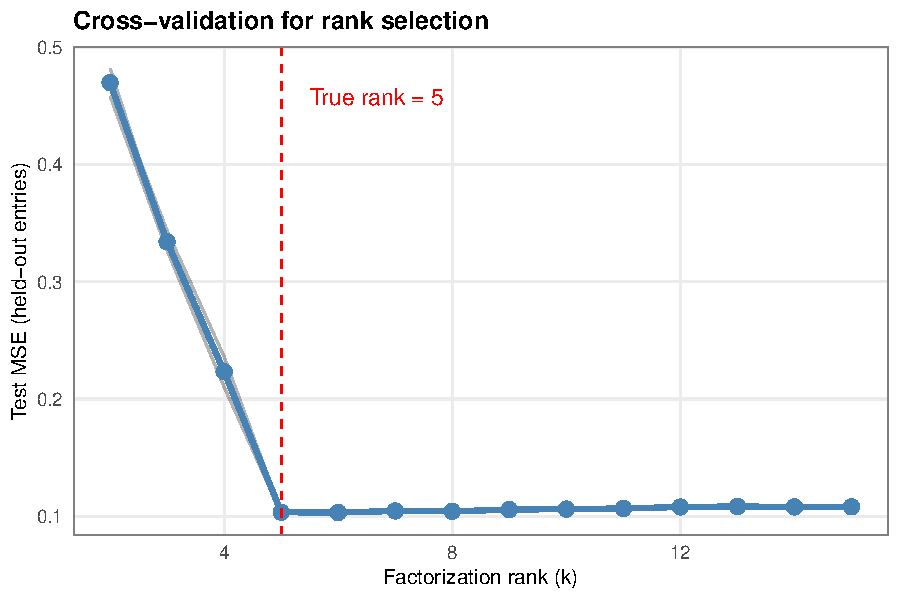
\includegraphics[width=0.8\textwidth]{fig_cv_rank}
\caption{\label{fig:cv}Cross-validation for rank selection on synthetic data 
with true rank 5. Test MSE is minimized near the true rank.}
\end{figure}

\subsection{Regularization effects}

Figure~\ref{fig:l1} shows the trade-off between reconstruction error and 
factor sparsity under L1 regularization.

\begin{figure}[t]
\centering
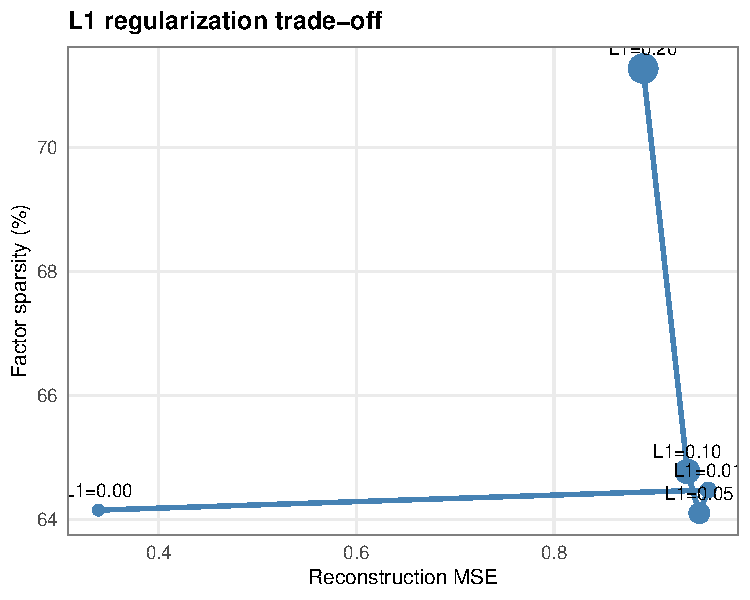
\includegraphics[width=0.7\textwidth]{fig_l1_tradeoff}
\caption{\label{fig:l1}L1 regularization trade-off.}
\end{figure}

\subsection{Scaling behavior}

Figure~\ref{fig:scaling} shows runtime scaling for sparse and dense matrices.

\begin{figure}[t]
\centering
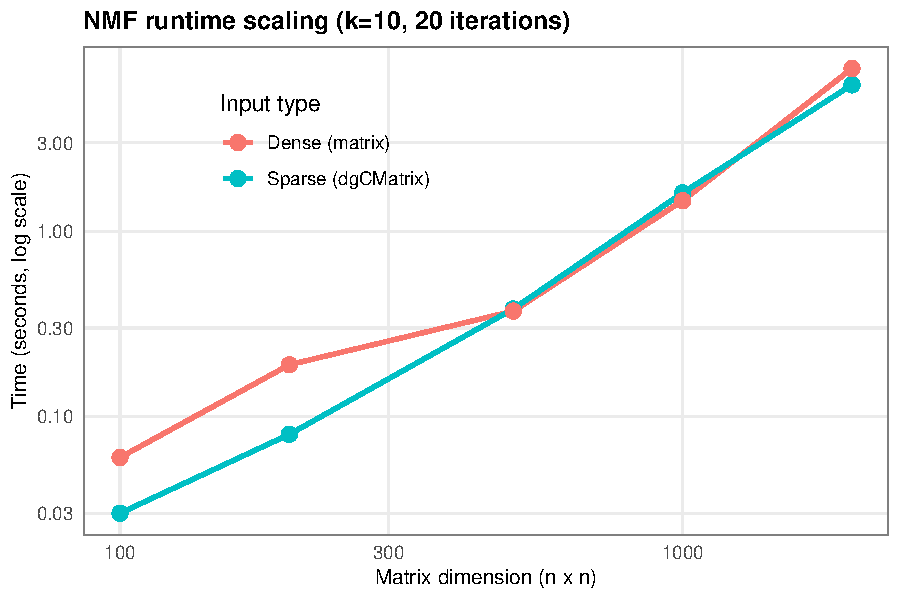
\includegraphics[width=0.8\textwidth]{fig_scaling}
\caption{\label{fig:scaling}Runtime scaling for NMF on sparse and dense matrices.}
\end{figure}


%% =============================================================================
\section{Summary} \label{sec:summary}

The \pkg{RcppML} package provides a comprehensive NMF implementation for 
\proglang{R} with integrated cross-validation, multiple loss functions via IRLS, 
automatic rank determination through golden section search, and specialized 
rank-2 NMF for spectral bipartitioning. The package is available on CRAN.


%% -- Computational details ----------------------------------------------------

\section*{Computational details}

The results in this paper were obtained using \proglang{R}~4.5.0 with the 
packages \pkg{RcppML}~1.0.0, \pkg{Matrix}~1.7.3, \pkg{irlba}~2.3.5.1, and 
\pkg{ggplot2}~4.0.1.


%% -- Bibliography -------------------------------------------------------------

\bibliographystyle{plainnat}
\bibliography{refs}

\end{document}
